%%%%%%%%%%%%%%%%%%%%%%%%%%%%%%%%%%%%%%%%%
% Beamer Presentation
% LaTeX Template
% Version 1.0 (10/11/12)
%
% This template has been downloaded from:
% http://www.LaTeXTemplates.com
%
% License:
% CC BY-NC-SA 3.0 (http://creativecommons.org/licenses/by-nc-sa/3.0/)
%
%%%%%%%%%%%%%%%%%%%%%%%%%%%%%%%%%%%%%%%%%

%----------------------------------------------------------------------------------------
%	PACKAGES AND THEMES
%----------------------------------------------------------------------------------------

\documentclass{beamer}

\mode<presentation> {

\usetheme{Madrid}

}

\definecolor{DataBlue}{rgb}{0.50, 0.85, 0.99} 

\setbeamercolor{titlelike}{parent=structure,bg=black, fg = white}
\setbeamercolor{frametitle}{fg=white}
\usepackage{graphicx} % Allows including images
\usepackage{booktabs} % Allows the use of \toprule, \midrule and \bottomrule in tables
\usepackage[export]{adjustbox}


%----------------------------------------------------------------------------------------
%	TITLE PAGE
%----------------------------------------------------------------------------------------

\title{EE4013 - C and Data Structures} %% Title
\author{} % Your name
\author{Tejaswini A V \\ EE18BTECH11047}
%\institute[USP] % Your institution as it will appear on the bottom of every slide, may be shorthand to save space
\date{October 13, 2021}

% Rodapé
\setbeamertemplate{footline}{%
    \begin{beamercolorbox}[wd=\paperwidth]{footlinecolor}
        %\includegraphics[width=\paperwidth]{images/footbar.png}
    \end{beamercolorbox}%
}

\begin{document}
{
\setbeamertemplate{footline}{} 
\begin{frame}
\titlepage
\end{frame}
}

\begin{frame}{Data structure - Queue}
\textbf{Problem: } A queue is implemented using a non-circular singly linked list. The queue has a head pointer and a tail pointer, as shown in the figure. Let \emph{n} denote the number of nodes in the queue. Let \emph{enqueue} be implemented by inserting a new node at the head, and \emph{dequeue} be implemented by deletion of a node from the tail.

\begin{figure}[!ht]
    \begin{center}
    \includegraphics[width=90mm,scale=1]{figs/queue}
    \end{center}
    \label{fig:roc}	
\end{figure}

What is the time complexity of the most time-efficient implementation of \emph{enqueue} and \emph{dequeue}, respectively, for this data structure?
\end{frame}

\begin{frame}{Solution - Enqueue}

\textbf{Enqueue:} The enqueue operation involves two operations:
\begin{itemize}
    \item Create a new node with the value to be inserted and point the next pointer of this node to the head of the linked list.
    \item Make the new node as the head of the linked list.
\end{itemize}
Creating a new node and changing two pointers can be performed in constant time. Therefore, time complexity of \emph{enqueue} operation is $\Theta (1)$ .
    
\end{frame}

\begin{frame}{Enqueue - Time complexity}
The following plot shows the experimental time complexities of Enqueue operation for various values of n.
\begin{figure}[!ht]
    \begin{center}
    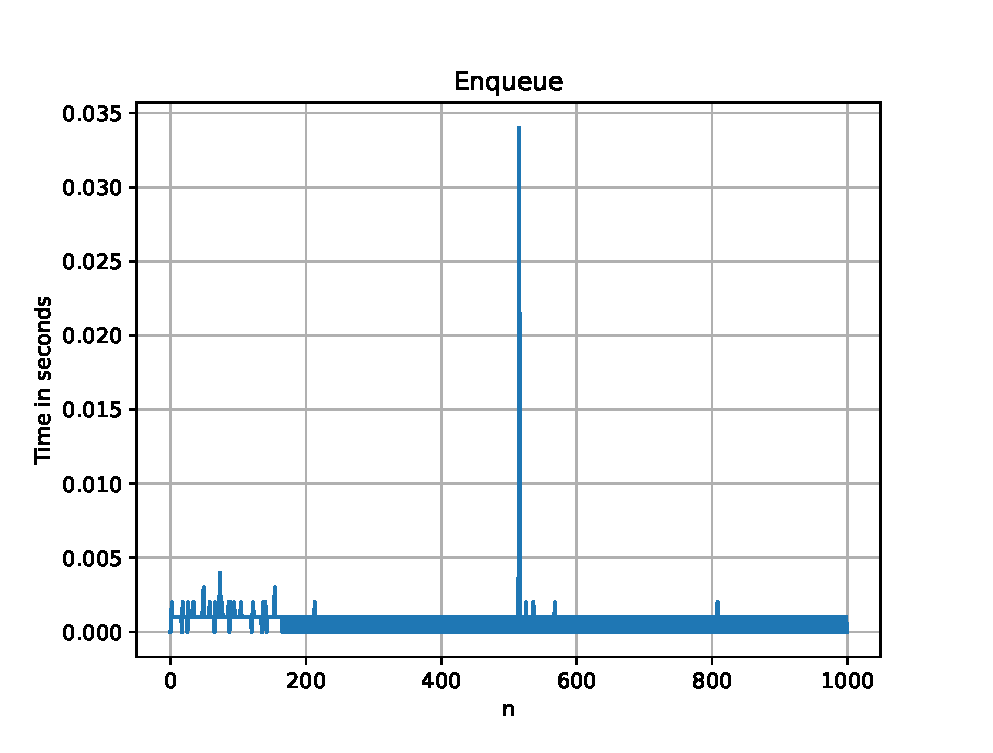
\includegraphics[width=80mm,scale=0.8]{./figs/enqueue}
    \end{center}
    \label{fig1}	
\end{figure}
    
\end{frame}


\begin{frame}{Dequeue}
\textbf{Dequeue: } The dequeue operation involves the following steps:
\begin{itemize}
    \item Delete the tail node.
    \item Traverse the linked list to find the address of the second last node and make the next pointer NULL. Update the tail pointer.
\end{itemize}

Since we are traversing the whole linked list, the time 
complexity of \emph{dequeue} operation is $\Theta (n)$ where n is the number of nodes in the linked list.
    
\end{frame}


\begin{frame}{Dequeue - Time complexity}
The following plot shows the experimental time complexities of Dequeue operation for various values of n.
\begin{figure}[!ht]
    \begin{center}
    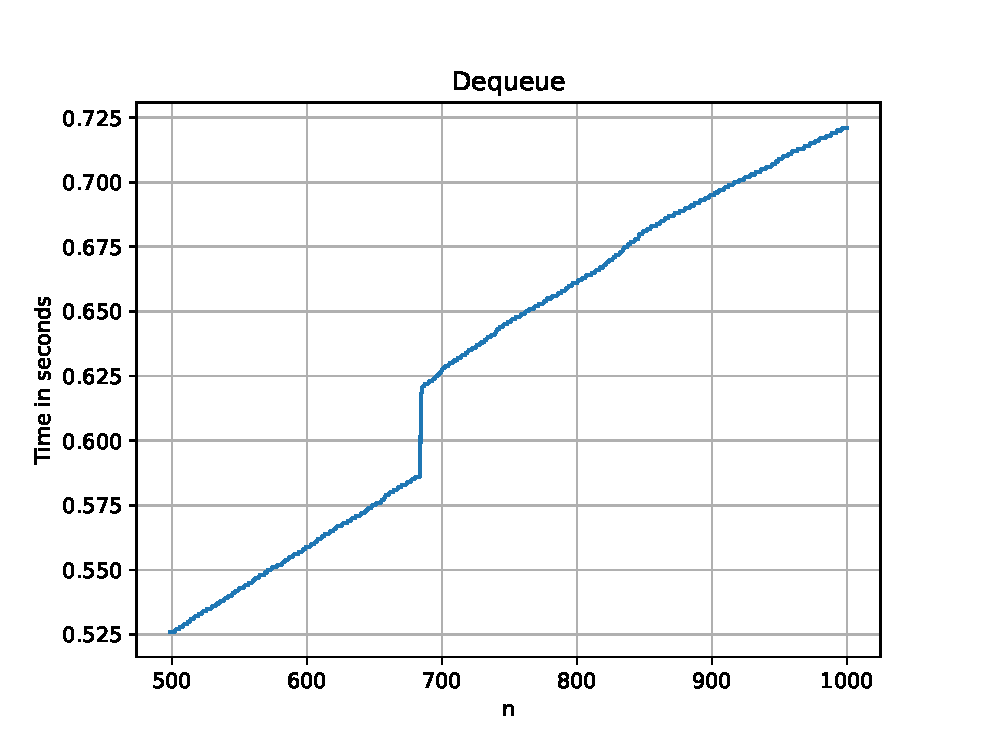
\includegraphics[width=80mm,scale=0.8]{./figs/dequeue}
    \end{center}
    \label{fig2}	
\end{figure}
    
\end{frame}

\begin{frame}{Time complexity}
Range of time taken: 
\\
\textbf{Enqueue} -  $[0.156, 0.412]$ $\mu$ sec
\\
\textbf{Dequeue} - $[5.356, 12.756]$ $\mu$ sec
\\
Approximate equation of the time taken by dequeue is

\begin{align}
    n_{1} = 500; t_{1} = 5.356 \mu sec  
\\
    n_{2} = 1000; t_{2} = 12.756 \mu sec
\\
    slope(m) = \frac{t_{2}-t_{1}}{n_{2}-n_{1}} = 0.0148
\end{align}
\begin{equation}
    Intercept(c) = t_{1} - m*n_{1} = 5.356 - 0.0148*500 = -2.044
\end{equation}
\begin{equation}
    \implies t = m*n + c
\end{equation}
\begin{equation}
    \implies t = 0.0148*n - 2.044
\end{equation}
where $n$ is the number of nodes in the linked list and $t$ is the corresponding time taken for dequeue operation in micro seconds($\mu$ secs).

    
\end{frame}

\begin{frame}{Conclusion}
Therefore, the time complexity of the most time efficient implementation of \emph{enqueue} and \emph{dequeue} respectively are $\Theta(1)$ and $\Theta(n)$.
    
\end{frame}
\end{document}